\section{
    Resumo do livro \textit{A Terceira Onda}, do Alvin Toffler
    }

\setlength{\parindent}{4em}
\setlength{\parskip}{0.5em}
\renewcommand{\baselinestretch}{1}



%\begin{figure}[h]
%    \centering
%    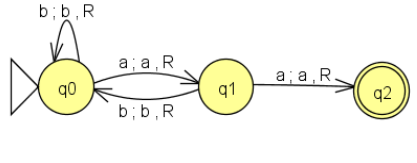
\includegraphics[width=0.65\textwidth]{ex1.png}
%    \caption{Máquina de Turing M.}
%    \label{fig:ex1}
%\end{figure}
%
%A linguagem reconhecida pela MT M é a das cadeias em \begin{math} \Sigma^* = \{a,b\}\end{math} que terminem com a subcadeia \begin{math} aa \end{math}. A expressão regular que define essa linguagem, pode ser a seguinte:
%\begin{center}
%    \begin{math}
%        (b^*a)^+a
%    \end{math}
%\end{center}